% !TeX encoding = UTF-8
% !TeX program = xelatex
% !TeX spellcheck = en_US

\documentclass[a4paper]{ltxdoc}
\usepackage{amsmath}
\usepackage[UTF8]{ctex}
\usepackage{unicode-math}
\usepackage{caption}
\usepackage{booktabs}
\usepackage{xcolor}
\usepackage{array}
\usepackage{listings}
\usepackage[perpage]{footmisc}
\usepackage{hypdoc}
\usepackage{geometry}
\usepackage{endnotes}
\usepackage{graphicx}
% \usepackage[multiple]{endnotes}
\usepackage{multicol}
\usepackage{listings}
\usepackage{hyperref}
\usepackage{blindtext}
\usepackage{palatino}
\usepackage{tikz}
\setmainfont{TeX Gyre Termes}
\usetikzlibrary{shapes.geometric, arrows}
\geometry{a4paper, scale=0.85}
\lstset{
    basicstyle          =   \sffamily,          % 基本代码风格
    keywordstyle        =   \bfseries,          % 关键字风格
    commentstyle        =   \rmfamily\itshape,  % 注释的风格,斜体
    stringstyle         =   \ttfamily,  % 字符串风格
    flexiblecolumns,                % 别问为什么,加上这个
    numbers             =   left,   % 行号的位置在左边
    showspaces          =   false,  % 是否显示空格,显示了有点乱,所以不现实了
    numberstyle         =   \zihao{-5}\ttfamily,    % 行号的样式,小五号,tt等宽字体
    showstringspaces    =   false,
    captionpos          =   t,      % 这段代码的名字所呈现的位置,t指的是top上面
    frame               =   lrtb,   % 显示边框
}
\lstdefinestyle{Python}{
    language        =   Python, % 语言选Python
    basicstyle      =   \zihao{-5}\ttfamily,
    numberstyle     =   \zihao{-5}\ttfamily,
    keywordstyle    =   \color{blue},
    keywordstyle    =   [2] \color{teal},
    stringstyle     =   \color{magenta},
    commentstyle    =   \color{red}\ttfamily,
    breaklines      =   true,   % 自动换行,建议不要写太长的行
    columns         =   fixed,  % 如果不加这一句,字间距就不固定,很丑,必须加
    basewidth       =   0.5em,
}

\thispagestyle{empty}
\tikzstyle{startstop} = [rectangle, rounded corners, minimum width = 2cm, minimum height=1cm,text centered, draw = black]
\tikzstyle{io} = [trapezium, trapezium left angle=70, trapezium right angle=110, minimum width=2cm, minimum height=1cm, text centered, draw=black]
\tikzstyle{process} = [rectangle, minimum width=3cm, minimum height=1cm, text centered, draw=black]
\tikzstyle{decision} = [diamond, aspect = 3, text centered, draw=black]
\tikzstyle{arrow} = [->,>=stealth]


\title{基于SEIR模型的传染病模拟分析}
\author{少年班学院\ \ 马天开\ \ PB21000030}
\date{\today}

\begin{document}
\maketitle
\section{科学技术原理}
\textit{SEIR}模型是一种基本的传染病模型,其在\textit{SIR}模型基础上发展得到。它将传染过程分为了如下几个阶段:

\begin{itemize}
    \item S,susceptible,即易感人群,存在感染风险
    \item E,exposed,即携带者,体内存在病毒,但并不具有传染性。经过一段时间后会变为感染者。
    \item I,infected,即感染者,具有传染性。存在治愈率和致死率。
    \item R,recovered,即恢复者,已经治愈,在\textit{SEIR}模型中,假定免疫是不会消失的(即不会重新变为易感人群)。
\end{itemize}


\begin{figure}[h]
    \centering
    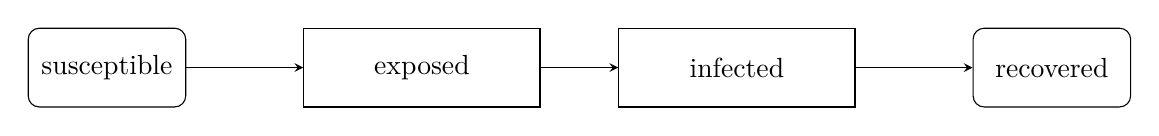
\begin{tikzpicture}[node distance=4cm]
        \node (start) [startstop]{susceptible};
        \node (pro1) [process, right of = start] {exposed};
        \node (pro2) [process, right of = pro1] {infected};
        \node (pro3) [startstop, right of = pro2] {recovered};
        \draw [arrow] (start) -- (pro1);
        \draw [arrow] (pro1) -- (pro2);
        \draw [arrow] (pro2) -- (pro3);
    \end{tikzpicture}
\end{figure}

在这个模型中,出于方便考虑可以做如下假设:
\begin{itemize}
    \item 自然出生率$\mathbb \Lambda$与死亡率$N\mu$相同(意为总人口$N = S + E + I + R$保持不变,但依然假定死亡率存在)
    \item 从被感染到发病存在一个间隔,参数表示为$a\ days^{-1}$(意为平均发病间隔时间为$a ^{-1} days$)
\end{itemize}

由以上内容,可以导出这个模型的一般方程:

\begin{equation}
    \left\{
    \begin{aligned}
        \dfrac {dS} {dt} & = \mu N - \mu S - \dfrac {\beta IS }{N} \\
        \dfrac {dE} {dt} & = \dfrac {\beta IS} {N} - (\mu + a)E    \\
        \dfrac {dI} {dt} & = aE -(\gamma + \mu)I                   \\
        \dfrac {dR} {dt} & = \gamma I - \mu R                      \\
    \end{aligned}
    \right.
\end{equation}

在此基础上改进的模型还包括:\textit{SEIRS}、\textit{MSEIR}、\textit{MSEIRS}等,其中\textit{M}群体的引入是考虑到部分传染病在婴儿身上天然免疫的情况,而\textit{SEIRS}退化的引入则是考虑到部分传染病存在免疫的时效性,康复人群有概率消失掉已经获得的免疫。

针对\textit{covid-19},上述两种情况对结果的影响都足够小,可以忽略。值得注意的是,以上探讨的数学模型,虽然能很好地拟合现有数据,但却没有讨论人群流动对于传播速度的影响。具体来说,是流动对于$\alpha$值的改变,在这里我们给出一个最直观的表述。

本程序通过一种简单网格状的模拟,希望给出流动对于传播速率的影响的一个简单分析。

\begin{figure}[h]
    \centering
    \includegraphics[scale = 0.3]{images/1.png}
    \caption{程序运行界面,其中左侧展示了当前各种状态的人数,右侧展示了随时间变化的曲线}
\end{figure}


在程序运行时,可以逐步观看传播的过程和右侧曲线变化,在模拟量足够大时,右侧曲线与模型一般方程推导的结论完全一致。

然而,当我们改变\textit{emulation\_move\_speed}的值时,既调整人口流动速度时,我们会发现,右侧曲线出现了较大的偏移。

\begin{figure}[h]
    \centering
    \includegraphics[scale = 0.3]{images/2.png}
    \caption{当模拟的流动速度增大时,传播曲线有着明显的变化}
\end{figure}

为了准确的刻画这种流动速度对传播结果带来的影响,我们引入一个评估的参考值:$round$,既使得$I$减半所需要花费的模拟周期数。

根据模拟计算,可以得到如下$round-speed$关系:

\begin{figure}[h]
    \centering
    \includegraphics[scale = 0.7]{images/3.png}
    \caption{减半周期随移动速度关系}
\end{figure}

可以看到,随着流动速度逐渐增大,流动速度对传播速度的增益逐渐放缓,在模拟的终点甚至有略微下降的趋势,在流动速度的起始位置有着最佳收益点。

\section{设计方案}

本项目利用了\textit{numpy}和\textit{matplotlib}作为基础,利用模拟的办法计算传播过程。

参考一篇文献中给出的参数,将系数初始值设定为:

\begin{equation}
    \left\{
    \begin{aligned}
        \alpha & = 0.62\times 10^{-7}  \\
        \beta  & = 1 / 14 \ days ^{-1} \\
        \sigma & = 0.000667            \\
        \mu_i  & = 7.344\times 10^{-7} \\
    \end{aligned}
    \right.
\end{equation}

\subsection{数据结构和初始化}

为方便处理,以及考虑到模拟需要,将数据存储为一个$(4*size*size)$的\textit{np.array}其中$axis=0$分别代表$S,E,I,R$的分布情况,\textit{size}为模拟的单元格数量。

在初始化时,考虑到人口的分布一般是集中的,因此采用了正态分布的方式进行模拟,在初始条件上,设定$I = S/2$来更快地得到模拟结果。

\subsection{\textit{Move}函数}

\textit{Move}函数主要负责模拟人群的流动,实现方式如下:\par

如果只考虑相邻单元格间人口的流动,可以采取以下方法:使用\textit{np.random.normal}生成一个$(4*4*size*size)$的矩阵,分别代表各个方向迁移的人口占比,每个数据均限制在$[0,0.25)$之间。然后通过\textit{np.roll}的方式偏移矩阵,叠加最终的结果到原始矩阵上。

\subsection{\textit{Spread}函数}

\textit{Spread}函数负责模拟各单元格内的传播,通过模拟单个周期内传播的人数来实现。

值得注意的是,按照传播模型计算的人数,是浮点数,并不符合模拟的要求。为此,编写了一个\textit{randFloatToInt}函数,将浮点数转化为整数,同时保留了统计意义上的期望值。

\section{创新性表述}

本文中提到的所有代码均为本人独立完成,在数据上借鉴了一篇相关的期刊,其余内容均为代码模拟得到。

\bigskip


创新点:

\begin{itemize}
    \item 在原传播模型的基础上,通过模拟的方法,讨论了流动对传播的影响。
    \item 通过图表的方式,直观的展现了疫情传播的过程。
    \item 通过对流动和传播结果之间的关系的讨论,具有一定的社会意义。
\end{itemize}

\section{运行方法和参数设置}

可以直接运行\textit{main.py}得到,在打开的命令窗口中敲击回车来模拟一轮计算。

同时,可以通过修改代码的方式得到想要的运行结果,例如可以通过调整\textit{while not reached:}为\textit{for i in range(1000)}来直接模拟运行100次后的结果。

参数设置方面,本程序系模拟程序,全部参数放在了代码的起始位置并可调,具体解释如下:

\begin{itemize}
    \item $size$,模拟单元格的数量,应该和人数保持对应关系
    \item $emulation\ p\ size$,模拟的人数,如遇性能问题应该适当降低
    \item $emulation\ scale$,人口的正态分布方差,越小人口分布越密集
    \item $emulation\ move\ speed$,人口的流动速度,越大流动越快
    \item $emulation\ initial\ infected$,初始的感染人数
    \item $rate$,模拟周期的倍率,可以适当调大来满足性能要求
    \item $value\ mu$,自然死亡率
    \item $value\ alpha$,传播率
    \item $value\ beta$,潜伏期的倒数
    \item $value\ sigma$,治愈率
    \item $value\ mu\  i$,病死率
\end{itemize}

\section{学习心得和收获}

经过本次课程的学习,更加熟练了有关\textit{Python}有关科学计算的包的应用和处理方式。对于各种\textit{IDE}的测试、\textit{matplotlib}等有了更进一步的掌握。

在本次课程之前,我对\textit{Python}一直处在一个自己摸索、时常碰壁的学习路上。在最开始使用的时候更为严重,平均下来写代码和排查错误的时间大概要对半分。也不能很好地利用报错信息来排查错误,导致我最开始使用Python的体验相当不好,甚至我一度怀疑这样一门语言对效率的提升究竟有多大。

在本次课程之后,尤其是从课程一开始我就在搞的这个项目,逐渐锻炼了我排查错误、调试以及熟练查文档的能力。现在能达到几乎写C++效率的3倍左右,可以说真正地把Python当作一个有趣的工具来使用,也希望它能在日后的学习/工作中更大地发挥作用。

具体一点讲的话,在本次项目中收获最大的应该要数Anaconda和Pycharm的使用了。有趣的工具总是能带来更有趣的体验。熟练使用之后,会比单纯使用VSCode的体验和速度更上一层楼。

\section{参考文献}

Suwardi Annas, Muh. Isbar Pratama, Muh. Rifandi, Wahidah Sanusi, Syafruddin Side, Stability analysis and numerical simulation of SEIR model for pandemic COVID-19 spread in Indonesia, Chaos, Solitons \& Fractals, Volume 139, 2020, 110072, ISSN 0960-0779

\end{document}